\newpage
\begin{center}
\noindent\textbf{ГЛАВА 1. РАСКРАСКИ СФЕР}\label{chapters:1}
\vspace{1.5mm}
\end{center}

\vspace{5pt}
\textbf{1.1 Постановка задачи и известные результаты}\label{chapters:1.1}
\vspace{5pt}

Графом называется пара $G=(V,~E)$, где $V$ - вершины графа, $E \subseteq \{\, (u,v) \mid u,v \in V \,\}$ - ребра графа. 
Хроматическим числом графа $\chi(G)$ называется минимальное число $k$ такое, что множество вершин $V$ можно разбить (покрасить) на $k$ 
непересекающихся классов $V_1 \sqcup V_1 \sqcup \dots \sqcup V_k = V$ так, что никакое ребро из $E$ не соединяет вершины одного класса. 
В данной работе рассматривается задача о хроматическом числе двумерной сферы 
$S^2(r) = \{\, x \in \mathbb{R}^3 : \|x\| = r \,\}$, сформулированная Полом Эрдёшем в 1981 году [\ref{bib:ErdosGraham}].
Предполагается, что расстояние между точками сферы $x,y \in S^2(r)$ задано евклидовой метрикой в $\mathbb{R}^3$: 
$d(x,y) = \sqrt{\sum_{i=1}^{3}(x_i-y_i)^2}$. Тогда 
$\chi(S^2(r)) = \min \{\, k: S^2(r) = V_1 \sqcup \dots \sqcup V_k , \, x,y \in V_i \Rightarrow \|x - y\| \ne 1 \,\}$. 
Во всех случаях, когда требуются непосредственные вычисления, предполагается, что центр сферы находится в начале координат.

Очевидно, что $\chi(S^2(r))$ зависит от $r$: если $r < \tfrac{1}{2}$, то $\chi(S^2(r))=1$, в то же время 
$S^2\left(\tfrac{1}{2}\right) = 2$ (подходит любая раскраска, в которой диаметрально противоположные точки имеют разный цвет).
При $r > \tfrac{1}{2}$ выполнено $\chi(S^2(r))>2$, так как соответствующий континуальный граф $G(S^2(r); 1)$ содержит нечетный цикл, для раскраски которого необходимы по крайней мере $3$ цвета.
В статье [\ref{bib:Simmons}] Симмонса был получен следующий результат:

\begin{theorem1}[Симмонс, 1976]
$$ \chi\left(S^2\left(\frac{1}{\sqrt{2}}\right)\right)=4, \quad \chi(S^2(r)) \geq 4 \text{ при } r > \frac{1}{\sqrt{3}}. $$
\end{theorem1}

Последнее неравенство было получено вложением в сферу конструкции, аналогичной \enquote{свернутому} веретену Мозера (\figurename{ \ref{chapter1:fig:simmons}}), для раскраски которой необходимо $4$ цвета. 
Отметим, что раскраска сферы $\chi\left(S^2\left(\frac{1}{\sqrt{2}}\right)\right)$ возникает в некой задаче квантовой механики, вследствие чего этот результат был переоткрыт другими авторами. Случай интересен тем, что $d(u,v)=1$ эквивалентно $(u,v)=0$ .
Из неравенства $\chi(\mathbb{R}^3) \leq 15$ следует, что 
$$\forall r>0 \quad \chi(S^2(r)) \leq 15.$$

\begin{figure}[h]
\centering
\captionsetup{justification=centering}
\begin{minipage}[h]{0.5\linewidth}
\center{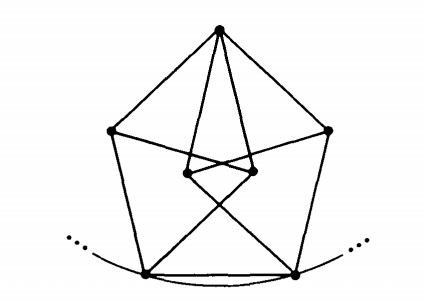
\includegraphics[width=0.4\paperwidth]{chapters/chapter1/simmons2.png}}
\end{minipage}\hfill
\begin{minipage}[h]{0.5\linewidth}
\center{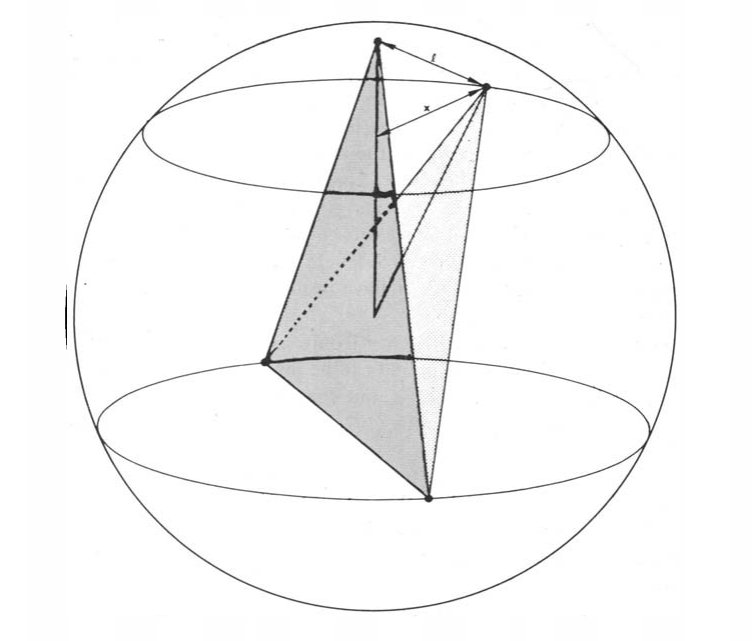
\includegraphics[width=0.4\paperwidth]{chapters/chapter1/simmons.png}}
\end{minipage}\hfill
\caption{К теореме Симмонса.}
\label{chapter1:fig:simmons}
\end{figure}

В дополнение к предыдущим рассмотрим некоторые асимптотические оценки и оценки для . В 1983 году  Л. Ловас доказал, что  $\chi(S^{n-1}(r)) \geq n$. В статье [\ref{bib:RaiSphere}] А.М. Райгородским показал, что хроматическое число сферы растет экспоненциально при росте размерности для всех $r > \frac{1}{2}$.

\begin{theorem1}

$$\text{Если } r \in (\frac{1}{2}, \frac{1}{\sqrt{2}}], \text{ то } 
\chi(S^{n-1}(r)) \geq \left(2(\frac{1}{8r^2})^{\frac{1}{8r^2}}(1-\frac{1}{8r^2})^{1-\frac{1}{8r^2}}+o(1)\right)^n.$$ 

$$\text{Если } r \geq \frac{1}{\sqrt{2}}, \text{ то } 
\chi(S^{n-1}(r)) \geq \left(2(\frac{1}{4})^{\frac{1}{4}}(\frac{3}{4})^{\frac{3}{4}}+o(1)\right)^n.$$

\end{theorem1}
В работе [\ref{bib:Kostina}] О. Костина доказала усиленный вариант предыдудщей теоремы.

\begin{theorem1}
Пусть $r > \tfrac{1}{2}$ и $b_1, b_{-1}$ таковы, что $b_1 + b_{-1} \in (0,1]$ и $b_1 < b_{-1}$.
Пусть $k_1=[b_1n]$ и $k_{-1}=[b_{-1}n]$. Положим

$$p_0(r,b_1,b_{-1},n) = \frac{(k_1 + k_{-1})n - (k_1 + k_{-1})^2}{2nr^2}$$
Пусть $p(r,b_1,b_{-1},n)$ - минимальное простое число, строго большее, чем $p_0$. 
Если при данных $r,b_1,b_{-1},n$ выполнено $k_1 + k_{-1} - 2p < -2k_{-1}$, то

$$\chi(S^{n-1}(r)) \geq 
\frac{\binom{n}{k_1}\binom{n-k_1}{k_{-1}}}
{\sum\limits_{(m_1,m_2) \in \mathcal{A}} \binom{n}{m_1} \binom{n-m_1}{m_2}}$$
где $\mathcal{A} = \{ (m_1,m_2): m_1,m_2 \in \mathbb{N} \cup \{ 0 \}, m_1+m_2 \leq n, m_1+2m_2 \leq p-1 \}$.

\end{theorem1}

Очевидно, что $\chi(S^{n-1}(r)) \leq \chi(\mathbb{R}^n) \leq (3+o(1))^n$, т.к. $S^{n-1}(r)$ лежит в $\mathbb{R}^n$. В общем случае лучших верхних оценок нет. Однако К.А. Роджерс [\ref{bib:Rogers}] получил более точную оценку в случае $r < \frac{3}{2}$.

\begin{theorem1}
$$\text{Если } r < \frac{3}{2}, \text{ то } \chi(S^{n-1}(r)) \leq (2r+o(1))^n.$$
\end{theorem1}

В работе [\ref{bib:Pros}] Р. Просановым получена следующая верхняя оценка хроматического числа сферы:

\begin{theorem1}
$\chi(S_r^{n-1}) \leq (x(r)+o(1))^n$, где
$$ x(r) = 
\begin{cases}
\sqrt{5-\frac{2}{r}+4\sqrt{1-\frac{5r^2-1}{4r^4}}},& \quad r > \frac{\sqrt{5}}{2} \\ 
2r,& \quad \frac{1}{2} < r \leq  \frac{\sqrt{5}}{2}
\end{cases}.$$
\end{theorem1}

\vspace{5pt}
\textbf{1.2 Разбиение на области Вороного}\label{chapters:1.2}
\vspace{5pt}

\vspace{5pt}
\textbf{1.3 Сферическая диаграмма Вороного}\label{chapters:1.3}
\vspace{5pt}